\section{Theory}
\label{sec:theorie}

Before discussing how interferometers work and how they can be used for precise measurements, we first need to cover some basics.

\subsection{Coherence}
\label{subsec:coherence}

Light propagates through space as waves with specific wavelength, thereby frequency and energy, amplitude and direction. 
Additionally, it is associated with a phase $\phi$ and polarisation (see \autoref{subsec:polarisation}).
Two light beams with energy $E_1$ and $E_2$ are called coherent if their difference in phase remains constant.
More specifically, coherence can be separated into spatial and temporal coherence.
If the beams' phase is predictable even for infinitely progressing time, we speak of temporal coherence.

If the difference in phase along one of the axes perpendicular to the propagation direction remains constant, we speak of spatial coherence.
Spatial coherence is essential in order for light to interfere.

In reality, all light has a coherence time $\tau_c$ and coherence length $l_c$ after which the temporal and spatial coherence is significantly reduced.


\subsection{Polarisation}
\label{subsec:polarisation}

Polarisation describes how the electric and magnetic fields oscillate with respect to the the light's direction of propagation.
There a three different general cases of polarisation: unpolarised light, where all field components oscillate in different directions, circularly polarised light,
where the fields oscillates in a circular motion around the propagation vector $\vec{k}$ and finally, most relevant for this experiment, linearly polarised light, where
the fields oscillate perpendicular to $\vec{k}$ in a fixed plane.


\subsection{Interference}
\label{subsec:interference}

If two beams of light with the same wavelength meet, they can interfere with each other.
In order for interference to occur, the two beams have to be spatially coherent as well as show parallel polarisation to each other.
Then, depending on what parts of the two waves interfere, the two amplitudes can either be amplified or weakened, if not entirely canceled out.


\subsection{Sagnac Interferometer}
\label{subsec:sagnacinterferometer}

The Sagnac Interferometer and other interferometers use interference to allow precise measurements of material specific values.

Here, the light source is a HeNe-laser.
The light is deflected by two mirrors and then passes through a polarisation filter into the polarising beam splitter cube (PBSC), 
a cube made of two prisms that deflects perpendicularly polarised light and lets parallely polarised light pass through without loss in intensity.
It splits up the beam into two perpendicular beams of light that continue to propagate through the aperture.
As can be seen in \autoref{fig:sagnac} below, the three other mirrors reflect the light around and finally out of the PBSC, 
where they emerge again as a single beam of light which is the projected onto a screen or enters the photo diodes.

\begin{figure}[H]
    \centering
    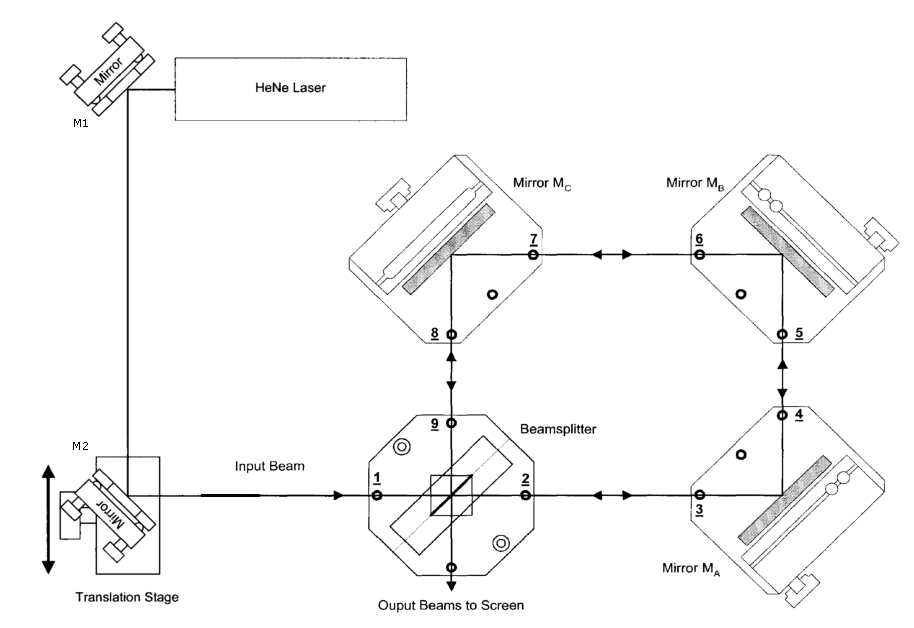
\includegraphics[width=\textwidth]{figures/V64_aufbau.pdf}
    \caption{Schematic representation of the aperture \cite{v64}.}
    \label{fig:sagnac}
\end{figure}

While interferometers like the Michelson- and Mach-Zehnder-Interferometer are quite sensitive to outside influences, the Sagnac Interferometer is much more stable
since, different from the other two mentioned interferometers, the two beams of light take the exact same path.

To conduct measurements, one of the two beams can be moved horizontally and then be sent through a gas cell or different medium that is to be inspected.
By then observing the interference of the beams after exiting the interferometer, we can derive values such as the refractive index.


\subsection{Contrast}

For that, we use the contrast $K$ of the Sagnac Interferometer.
With minimum intensity $I_{\text{min}}$ and maximum intensity $I_\text{max}$, it is defined as 
\begin{equation}
    K = \frac{I_\text{max} - I_\text{min}}{I_\text{max} + I_\text{min}} \in [0, 1] \,.
    \label{eq:contrast}
\end{equation}

Here, we are particularly interested in how the contrast depends on the polarisation angle $\varphi$. \\

Take
\begin{align*}
    I &\propto \langle | E_1 \cos(\omega t) + E_2 \cos(\omega t + \delta) | \rangle \\
      &= \langle E^2_1 \cos^2(\omega t) + E^2_2 \cos^2(\omega t + \delta) + 2 E_1 E_2 \cos(\omega t) \cos(\omega t + \delta) \rangle \\
      &= \frac{E^2_1 + E^2_2}{2} + E_1E_2 \cos(\delta)
\end{align*}
with 
\begin{align*}
    \langle \cos(\omega t) \rangle = \langle \cos(\omega t + \delta) \rangle &= \frac{1}{2} \\
    \langle \cos(\omega t) \cos(\omega t +\delta) \rangle &= \frac{1}{2} \cos(\delta)
\end{align*}
and $I_\text{Laser} \propto E^2_1 + E^2_2$ to derive a proportionality for $I_\text{min}$ and $I_\text{max}$
by plugging in the minimum and maximum values for $\cos(\delta)$ at $\delta=0$ and $\delta=\frac{\pi}{2}$ respectively. \\

We get
\begin{align*}
    I_{\text{max}/\text{min}} &\propto E^2_1 +E^2_2 \pm 2 \frac{E_1}{\sqrt{E^2_1 + E^2_2}} \frac{E_2}{\sqrt{E^2_1 + E^2_2}} (E^2_1+E^2_2) \\
    &\propto I_\text{Laser} (1 \pm 2 \sin(\varphi) \cos(\varphi))
\end{align*}
with $\cos(\varphi) = \frac{E_1}{\sqrt{E^2_1 + E^2_2}}$ and $\sin(\varphi) = \frac{E_2}{\sqrt{E^2_1 + E^2_2}}$ from geometric consideration,
leading to
\begin{align}
    K &\propto \left| \frac{1 + 2 \sin(\varphi) \cos(\varphi) - 1 - 2 \sin(\varphi) \cos(\varphi)}{1 + 2 \sin(\varphi) \cos(\varphi) + 1 - 2 \sin(\varphi) \cos(\varphi)}\right| \nonumber\\
      &\propto |\sin(2 \varphi)| \,.
      \label{eq:contrastprop}
\end{align}


\subsection{Interference and Refractive Index}
\label{subsec:intrefrac}

To measure the refractive indexes of glass and air, we need the relation between the number of interference maxima or minima $M$ and the difference in phase $\Delta\varphi$
created by the medium we want to analyse.

It is given by
\begin{equation}
    M = \frac{\Delta \varphi}{2 \pi}\,,
    \label{eq:intmax}
\end{equation} 
as seen in \cite{v64}.

\subsubsection{Refractive Index of Glass}

The difference in phase in glass is created by the lower propagation speed and the additional path the light has to travel as it is refracted off the surface.
As per \cite{v64}, the difference in phase follows
\begin{equation*}
    \Delta \varphi (\theta) = \frac{2 \pi}{\lambda_\text{vac}} T \left(\frac{n-1}{2n} \theta^2 + \mathcal{O}(\theta^4) \right)
\end{equation*}
with wavelength in vacuum $\lambda_\text{vac}$, glass thickness $T$ and refractive index $n$.
Here, we use two glass plates rotated by $10°$ to each other, yielding
\begin{equation*}
    \Delta \varphi(\theta) = \frac{\pi (n-1)}{\lambda_\text{vac} n}T \left((\theta + 10°)^2 - (\theta - 10°)^2\right)
\end{equation*}
and thereby a number of interference maxima
\begin{equation}
    M = 2 \, \frac{n-1}{\lambda_\text{vac} n} \, T \, \theta \cdot 10°
\end{equation}
an refractive index of
\begin{equation}
    n = \frac{1}{1 - \frac{M \lambda_\text{vac}}{2 \, T \, \theta \cdot 10°}}
    \label{eq:refractiveindexglass}
\end{equation}

\subsubsection{Refractive Index of Air}

In air, a phase shift of
\begin{equation*}
    \Delta \varphi = \frac{2 \pi}{\lambda_\text{vac}} \Delta n L 
\end{equation*}
is created, in turn causing
\begin{equation*}
    M = \frac{\Delta n L}{\lambda_\text{vac}}
\end{equation*}
interference maxima.
The refractive index is
\begin{equation*}
    n = 1 + \frac{M \lambda_\text{vac}}{L} \,.
\end{equation*}

Other than glass, air is a gas. 
Therefore, the number of interference maxima and thereby the refractive index is pressure dependant.
We use the Lorentz-Lorenz-law as in \cite{lololaw} to describe the pressure dependance as
\begin{equation*}
    \frac{n^2 - 1}{n^2 + 2} = \frac{1}{3} \frac{\alpha p}{\varepsilon_0 k_\text{B} T}
\end{equation*}
at pressure $p$ and temperature $T$.

For diluted gases, $n^2 + 2 \approx 3$ holds, yielding
\begin{equation*}
    n = \sqrt{\frac{\alpha p}{\varepsilon_0 k_\text{B} T} + 1}
\end{equation*}
or
\begin{equation}
    n \approx 1 + \frac{\alpha p}{2 \varepsilon k_\text{B} T}
    \label{eq:refractiveindexair}
\end{equation}
when using the Taylor approximation $\sqrt{1 + x} \approx 1 + \frac{x}{2}$.




